% Kopfzeile beim Kapitelanfang:
\fancypagestyle{plain}{
%Kopfzeile links bzw. innen
\fancyhead[L]{\Large Vorlesung 28 (30.01.2013)}
%Kopfzeile rechts bzw. außen
\fancyhead[R]{}}
%Kopfzeile links bzw. innen
\fancyhead[L]{\Large Vorlesung 28 (30.01.2014)}
%Kopfzeile rechts bzw. außen
\fancyhead[R]{}
% **************************************************
\section{Beispiel: Die Gamma-Funktion}\label{14.19}
\emph{\href{https://de.wikipedia.org/wiki/Gamma-Funktion}{\underline{Gamma-Funktion}}: von \href{https://de.wikipedia.org/wiki/Leonhard_Euler}{\underline{Leonhard Euler}}, 1729}\nl
$n!$ (Fakultät) ist nur definiert für $n \in \N_0$.\\
Ziel: Funktion $\Gamma: (0,\infty) \to \R$ mit $\Gamma(n+1)=n!$ (Das heißt: $\Gamma$ interpoliert die Fakultät)

\subsection*{Definition}
$\Gamma(s) := \int_0^\infty x^{s-1} e^{-x} dx$, $s>0$, ist die \underline{Gamma-Funktion}.

\section*{Konvergenz des Integrals (beide Grenzen kritisch)}
\enk{
\item Auf $(0,1]$: $|x^{s-1}e^{-x}| \le x^{s-1} \forall x>0$\\
$\int_0^1 x^{s-1} dx$ konvergiert $\forall s>0$ (Beispiel \ref{14.16}) $\underset{\text{Majorantenk. \ref{14.17}}}{\Ra} \int_0^1 x^{s-1} e^{-x} dx$ konvergiert
\item Auf $[1,\infty)$: Vergleichsfunktion: $g(x) = e^{-\frac{x}{2}}$\\
$\int_1^\infty e^{-\frac{x}{2}} dx < \infty$ (Beispiel \ref{14.16})\\
$\lim_{x \to \infty} \frac{x^{s-1}e^{-x}}{e^{-\frac{x}{2}}} = \lim_{x \to \infty} \frac{x^{s-1}}{e^{\frac{x}{2}}} = 0$\\
$\underset{\text{Grenzwertk. \ref{14.18}}}{\Ra} \int_1^\infty x^{s-1}e^{-x} dx$ existiert
}

\phantomsection
\addcontentsline{toc}{section}{Eigenschaften der Gamma-Funktion}
\section*{Eigenschaften der Gamma-Funktion}\label{EigenschaftenGamma}
\en{
\item $\Gamma(1) = 1$
\item $\Gamma(s+1) = s \cdot \Gamma(s) \forall s>=$ (Funktionalgleichung)
\item $\Gamma(n+1) = n! \forall n \in \N_0$ ($\Gamma$ interpoliert die Fakultät)
}

\subsection*{Beweis}
\en{
\item $\Gamma(1) = \int_0^\infty e^{-x} dx = \lim_{R \to \infty} \int_0^R e^{-x} ex = \lim_{R \to \infty} \left(-e^{-x} \arrowvert_0^R\right)$
\item $0 < \eps < \R < \infty$: $\underbrace{\int_\eps^R \underset{f}{x^s} \underset{g'}{e^{-x}} dx}_{\to \Gamma(s+1)} \underset{\text{pktw. Int.}}{=} \underbrace{-x^s e^{-x} \arrowvert_\eps^R}_{\to 0} + s \cdot \underbrace{\int_\eps^R x^{s-1} e^{-x} dx}_{\to f(s)}$ (für $\eps \downarrow 0, R \to \infty$)\\
$\Ra \Gamma(s+1) = s \cdot \Gamma(s)$
\item $\Gamma(n+1) \underset{\text{FG}}{=} n \cdot \Gamma(n) \underset{\text{FG}}{=} n(n-1) \cdot \Gamma(n-1) = \ldots = n! \cdot \Gamma(1) = n!$
} \qed

\newpage

\begin{figure}
\centering
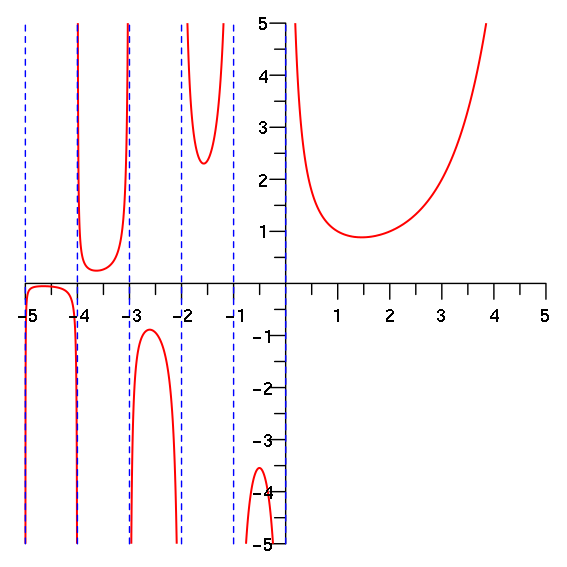
\includegraphics[scale=0.5]{img/2014-01-30/Gammafunktion}
\caption{Quelle: http://commons.wikimedia.org/wiki/File:Gammafunktion.svg}
%TODO: Wer eine Idee hat, wie man das mit tikz machen könnte, ich bin für Vorschläge offen. :)
\end{figure}

\subsection*{Bemerkung}
$\Gamma$ ist eine der wichtigsten Funktionen der Analysis, tritt oft in Normierungskonst. auf.

\phantomsection
\addcontentsline{toc}{section}{Stirlingsche Formel}
\section*{Stirlingsche Formel (Bemerkung zum Wachstum von $n!$)}
$n! \sim \sqrt{2 \pi n} \cdot \left(\frac{n}{e}a\right)^n$\nl
Dabei schreibt man für zwei Folgen $(a_n), (b_n) \subseteq \R$:\\
$a_n \sim b_n :\Lra \lim_{n \to \infty} \frac{a_n}{b_n} = 1$ (asymptotische Gleichheit)\nl
Hier: $\lim_{n \to \infty} \frac{n!}{\sqrt{2 \pi n} \cdot \left(\frac{n}{e}\right)^n} = 1$

\section{Integralkriterium}\label{14.20}
Sei $f: [1,\infty) \to \R$ monoton fallend, $f \ge 0$.\\
$a_n := \sum_{k=1}^n f(k) - \int_1^{n-1} f(x) dx$ ($n \in \N$)\nl
\begin{tikzpicture}
\draw[->] (-0.5,0)--(6,0);
\draw[->] (0,-0.5)--(0,2);
\draw[color=red,pattern=custom north west lines,hatchcolor=red] (0.5,0) -- (0.5,2) -- (1,2) -- (1,0) -- cycle;
\draw[color=red,pattern=custom north west lines,hatchcolor=red] (1,0) -- (1,1) -- (1.5,1) -- (1.5,0) -- cycle;
\draw[color=red,pattern=custom north west lines,hatchcolor=red] (2.5,0) -- (2.5,0.4) -- (3,0.4) -- (3,0) -- cycle;
\draw[color=red,pattern=custom north west lines,hatchcolor=red] (4.5,0) -- (4.5,0.22222222) -- (5,0.22222222) -- (5,0) -- cycle;
\draw[color=green,pattern=custom north west lines,hatchcolor=green] (0.5,2) -- plot [domain=0.5:1] (\x, {1/\x}) -- (1,2) -- cycle;
\draw[color=green,pattern=custom north west lines,hatchcolor=green] (1,1) -- plot [domain=1:1.5] (\x, {1/\x}) -- (1.5,1) -- cycle;
\draw[color=green,pattern=custom north west lines,hatchcolor=green] (2.5,0.4) -- plot [domain=2.5:3] (\x, {1/\x}) -- (3,0.4) -- cycle;
\draw[color=green,pattern=custom north west lines,hatchcolor=green] (4.5,0.22222222) -- plot [domain=4.5:5] (\x, {1/\x}) -- (5,0.22222222) -- cycle;
\draw[color=blue,domain=0.5:5] plot (\x, {1/\x});
\draw (0.5,0) node[below] {$1$} (1,0) node[below] {$2$} (1.5,0) node[below] {$3$} (2,0) node[below] {$\ldots$} (2.5,0) node[below] {\footnotesize $k$} (3,0) node[below] {\footnotesize $k+1$} (3.75,0) node[below] {$\ldots$} (4.5,0) node[below] {\footnotesize $n$} (5,0) node[below] {\footnotesize $n+1$};
\end{tikzpicture}\\
\emph{\footnotesize Der grüne Bereich entspricht $a_n$, der rote dem Integral und beide zusammen der Summe in obiger Gleichung}\nl
$\Ra \lim_{n \to \infty} a_n =: a$ existiert, und $0 \le a \le f(1)$\\
Ferner gilt: $\sum_{k=1}^\infty f(k)$ konvergiert $\Lra \int_1^\infty f(x) dx$ konvergiert
\subsection*{Beweis}
$f$ ist monoton fallend, $f \ge 0$.\nl
$(a_n)$ ist monoton wachsend und beschränkt mit $0 \le a_n \le f(1) \forall n$\\
$\Ra \lim_{n \to \infty} a_n = a$ existiert und $0 \le a \le f(1)$. Rest klar. \qed

\subsection*{Beispiel}
\en{
\item $f(x) = \frac{1}{x^s}, s>1$\\
$\int_1^\infty \frac{dx}{x^s}$ existiert $\Ra \sum_{n=1}^\infty \frac{1}{n^s}$ konvergiert\nl
\underline{Beachte}: $s \le 1 \Ra \sum_{n=1}^\infty \frac{1}{n^s}$ divergiert, da $\frac{1}{n^s} \ge \frac{1}{n}$ (harm. Reihe)\\
\^{=} $\int_1^\infty \frac{dx}{x^s}$ div. für $s<1$
\item $f(x) = \frac{1}{x} \Ra \lim_{n \to \infty} (\sum_{k=1}^n \frac{1}{k} - \ln(n+1)) =:  \gamma \in [0,1]$ existiert \emph{($\gamma$ ist die \href{https://de.wikipedia.org/wiki/Euler-Mascheroni-Konstante}{\underline{Euler-Mascheroni-Konstante}})}\\
d.h. $\sum_{k=1}^n \frac{1}{k} \sim \ln(n+1)$ für $n \to \infty$
}

\chapter{Taylorreihen}\label{P15}
\phantomsection
\addcontentsline{toc}{section}{Taylorpolynome}
\section*{Taylorpolynome}
Lineare Approximation einer differenzierbaren Funktion:\\
Sei $f: I \to \R$ differenzierbar in $a \in I$ und $I$ ein offenes Intervall.\nl
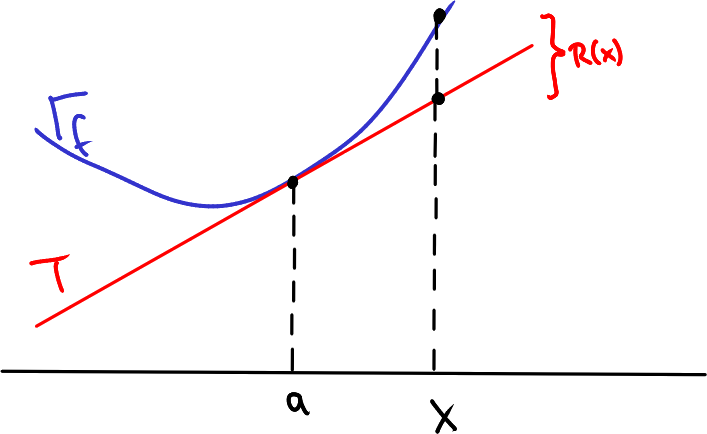
\includegraphics[scale=0.5]{img/2014-01-30/1}\nl %TODO: Vielleicht noch abtikzen?
Tangente an $\Gamma_f$ im Punkt $\underline{(a,f(a))}: T(x) = f(a)+f'(a)(x-a)$\nl
Wie gut ist diese Approximation in der Nähe von $a$?\\
Fehler: $R(x) = f(x)-T(x)$; $R(a) = 0$\\
$x \neq a \Ra \frac{R(x)}{x-a} = \underbrace{\frac{f(x)-f(a)}{x-a}}_{\to f'(a) \text{ für } x \to a} - f'(a) \Ra \lim_{x \to a} \frac{R(x)}{x-a} = 0$\nl
Das heißt, $R(x)$ geht für $x \to a$ deutlich schneller gegen $0$ als $x-a$.

\subsection*{Ziel}
Noch bessere Approximation durch Polynome höheren Grades, falls $f$ genug oft differenzierbar ist in $a$.\nl
Sei $f: I \to \R$ $n$-mal differenzierbar in $a \in I$, $I \subseteq R$ ein offenes Intervall.\\
Gesucht: Polynom $T$, grad $T \le n$, mit $T(a)=f(a)$, $T'(a)=f'(a)$, $T''(a)=f''(a)$, $\ldots$, $T^{(n)}(a) = f^{(n)}(a)$ (*)

\subsection*{Ansatz}
$T(x) = \sum_{k=0}^n c_k (x-a)^k$\\
$\Ra T(a) = c_0$, $T'(a)=c_1$, $T''(a)=2c_2$, $\ldots$, $T^{(n)}(a) = n! \cdot c_n$\\
$\Ra \exists!$ Polynom $T$ vom Grad $\le n$ mit (*), nämlich:
$$T_n f(x; a) = \sum_{k=0}^n \frac{f^{(n)}(a)}{k!} (x-a)^k$$
das \underline{Taylorpolynom} $n$-ter Ordnung an $f$ im Punkt $a$.\nl
$T_n f(x; a) = f(a) + f'(a) \cdot (x-a) + \frac{f''(a)}{2} \cdot (x-a)^2 + \ldots + \frac{f^{(n)}(a)}{n!} (x-a)^n$\nl
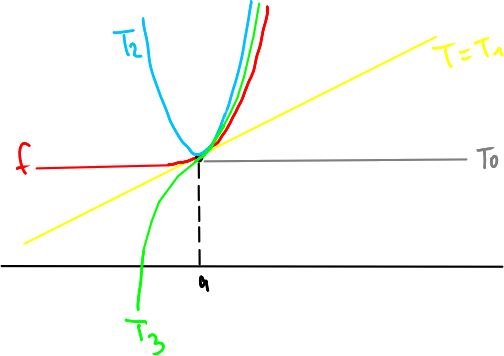
\includegraphics[scale=0.5]{img/2014-01-30/2}\nl %TODO: Vielleicht noch abtikzen?
$T_0 f$ hat den selben Wert wie $f$ in $a$\\
$T_1 f$ hat den selben Wert und die selbe Steigung\\
$T_2 f$ hat den selben Wert, die selbe Steigung und die selbe Krümmung\\
etc.

\subsection*{Beispiel}
$f(x) = \sqrt{1+x}$, $x \in (-1,1) \in I$ (bel. oft differenzierbar auf $I$)\nl
Taylorpolynom zweiter Ordnung von $f$ in $a=0$:\\
$f(0)=1$, $f'(x) = \frac{1}{2} (1+x)^{-\frac{1}{2}}$, $f'(0)=\frac{1}{2}$, $f''(x)=-\frac{1}{4} (1+x)^{-\frac{3}{2}}$, $f''(0) = -\frac{1}{4}$\\
$\Ra T_2 f(x;0) = 1 + \frac{1}{2} x - \frac{1}{8} x^2$

\subsection*{Beobachtung}
Approximationsgüte von $T_n f(x; a)$ nahe $a$?\\
Erwartung: Wird umso besser, je größer $n$ ist.

\subsection*{Restglied}
\fbox{$R_{n+1}(x) := f(x)-T_n f(x; a)$}

\newpage

\section{Satz: Integralformel für das Restglied}\label{15.1}
Sei $f \in C^{n+1} (I)$, $(n \in \N_0)$, $a \in I$ ($C^{n+1}(I)$ ist $n$-mal stetig differenzierbar auf $I$)\\
$\Ra$ \fbox{$R_{n+1}(x) = \frac{1}{n!} \int_a^x (x-t)^n f^{(n+1)}(t) dt$} $\forall x \in I$ (offenes Intervall)

\subsection*{Beweis mit Induktion nach $n$}
\items{
\item[$n=0$:] $R_1(x) = f(x)-f(a) \underset{\text{HDI}}{=} \int_a^x f'(t) dt$ \ok
\item[$n-1 \to n$:] $f(x)-T_{n-1} f(x; a) = R_n(x) \underset{\text{IV}}{=} \frac{1}{(n-1)!} \int_a^x (x-t)^{n-1} f^{(n)}(t) dt$\\
$\underset{\text{part. Int.}}{=} \underbrace{-\frac{(x-t)^n}{n!} f^{(n)} \arrowvert_a^x}_{=\frac{f^(n)(a)}{n!}(x-a)^n} + \frac{1}{n!} \int_a^x (x-t)^n f^{(n+1)}(t) dt$\nl
diesen Term nach links $\Ra$ Behauptung für $n$ \qed
}